\documentclass[a4paper]{article}

%%% packages %%%%%%%%%%%%%%%%%%%%%%%%%%%%%%%%%%%%%%%%%%%%%%%%%%%%%%%%%%%%%%%%%
\usepackage{graphicx}
\usepackage{subcaption}
\usepackage{amsmath,amssymb}
\usepackage{alltt}
\usepackage{natbib} % please use \citep and \citet instead of \cite
\usepackage{tikz}
\usetikzlibrary{positioning,automata}
\usetikzlibrary{shapes.geometric}
\usetikzlibrary{shapes.arrows}
\usepackage{array}
\usepackage{hyperref}
\usepackage{xcolor}
\usepackage{listings}
\usepackage[export]{adjustbox}

\definecolor{dark-red}{rgb}{0.4,0.15,0.15}
\definecolor{dark-blue}{rgb}{0.15,0.15,0.8}
\definecolor{medium-blue}{rgb}{0,0,0.5}
\hypersetup{
	colorlinks, linkcolor={dark-red},
	citecolor={dark-blue}, urlcolor={medium-blue}
}

\graphicspath{{./figs/}}
\DeclareGraphicsExtensions{.pdf}

\setlength{\parindent}{0mm}

\usepackage{fancyhdr}

%%% %%%%%%%%%%%%%%%%%%%%%%%%%%%%%%%%%%%%%%%%%%%%%%%%%%%%%%%%%%%%%%%%%%%%%%%%%

\makeatletter
\newcommand{\seminar}{Seminar Cyber-Physical Systems (WS 2019/20)}
\title{\textbf{Prioritized Sweeping Neural DynaQ:\\ Neural Networks over All?}}\let\Title\@title
\newcommand{\sTitle}{Prioritized Sweeping Neural DynaQ}
\newcommand{\AuthorName}{Alexander Osiik}
\author{\AuthorName\\
	\href{mailto:alexander.osiik@student.uni-luebeck.de}{alexander.osiik@student.uni-luebeck.de}\\
	\small \seminar\\
	%    \small Service Robotics Group\\
	\small Institute of Computer Engineering, University of L\"ubeck\\
}\let\Author\@author
\makeatother

\pagestyle{fancy}
\renewcommand{\footrulewidth}{0.4pt}
\lfoot{\seminar}
\cfoot{}
\rfoot{\thepage}
\lhead{\AuthorName}
\rhead{\sTitle}

%%% %%%%%%%%%%%%%%%%%%%%%%%%%%%%%%%%%%%%%%%%%%%%%%%%%%%%%%%%%%%%%%%%%%%%%%%%%

\begin{document}
	\maketitle
	
	\begin{abstract}
		\noindent%
		Reinforcement learning (RL) has gained a lot of popularity due to some spectacular successes. Q-learning is one of the most popular algorithms used for RL, where an agent builds an internal world model and action routine based on its interaction with the environment. However, the field of research becomes more and more complex and computationally demanding when trying to model naturally occurring psychological events and transfer them to artificial intelligence. Approaches including prioritized sweeping in dynamically growing neural networks were proposed, which are used to model and understand naturally occurring hippocampal replays, a memory consolidation process observed on rodents. This approach promises to improve the learning of simulated agents confronted a navigation task.
		Here we reproduced the performance results of \citet{NeuralDynaQ} regarding Q-learning for the same, minimally modified environment, after a short introduction to the state of the art of RL. It is also briefly outlined whether the development of a complex neural network is worthwhile for such a simple task, as the importance of comparative metric \textit{time} is often overlooked
	\end{abstract}
	
	
	\section{Introduction}
	In recent years, reinforcement learning (RL) has gained a lot of popularity due some spectacular successes \citep{Atari} . Reinforcement Learning is learning what to do based on the environment and how to map the situations into actions. Q-learning is one of the most popular algorithms used for RL, where an agent builds an action policy based on its interaction with the environment, without knowing anything about the state-transition and reward model. However, there is a clear limitation, as the computation and storage of such world models becomes infeasible in real unrestricted environments. \\
	To overcome this problem, neural networks are used. Learning in neural networks consists of finding and iteratively adjusting the right weights to approximate the needed value or policy function. \\
	Over the past years, different architectures for neural networks have been proposed to expertise them for specific problems or to improve the general performance \citep{James2018}. \citet{NeuralDynaQ} presented an approach including prioritized sweeping in dynamically growing neural networks, used to model naturally occuring hippocampal replays, a phenomenon observed on rodents. \\
	The content of this paper is divided into several parts. The introduction explains the biological background of \citet{NeuralDynaQ} work. Then, the basic mathematical concepts of reinforcment learning are reviewed. Ultimately, the performance of a self-developed Q-learning model is presented and evaluated regarding the results of \citet{NeuralDynaQ}.
	\subsection{Biological background}
	\label{sec:introduction}
	\par The hippocampus is the main memory of our brain and the switch point between short-term and long-term memory. \citet{OKEEFE1971171} observed in several rat experiments that if there is a disturbance in this area, no new information can be stored in the brain. Regarding animals, the hippocampus is known to be important for navigation since the discovery of place cells, which signal the current allocentric location of the animal in the environment \citep{Maguire}. Interaction within the environment leads to activation of these place cells. \cite{OKEEFE1971171} postulated that the hippocampus functions as a spatial map, where single hippocampal neurons increased their firing rate whenever a rat traversed a particular region of an environment, as concluded by \cite{Nakazawa}. They are engaged during the consolidation of spatial memories. However, it has been observed that these activations also occur during rest or sleep, at a significantly faster pace. This reactivation can be seen as a reprocessing of the experience gained during the day, something that is usually the case when dreaming \citep{HippocampalReplaysGirard}.
	
	\par \citet{NeuralDynaQ} presented an approach to convert the reactivation of the hippocampus' place cells into a reinforcement learning model.  
	
	\subsection{Experimental setup}
		\begin{figure}[t]
		\centering
		\includegraphics[angle=0,width=0.45\textwidth]{./figs/setup.png}
		\caption{\label{fig:setup}Discretized experimental setup. The agent has to make a decision at points T1 and T2, in which the decision at T2 leads to one of the rewarding sites. \citep{NeuralDynaQ}}
	\end{figure}
\par \cite{NeuralDynaQ} set up an experimental task, which was derived and slightly modified from \cite{GUPTA2010695}. The environment consisted of two successive T-mazes with lateral return corridors and rewarding food pellets on each side, see Figure \ref{fig:setup}. A rat was placed in the maze and trained to decide at position T2, intending to get the reward on the left or right-hand side based on the task pursued at the moment. The tasks were 1) always turn right, 2) always turn left, 3) alternate between left and right. At reward locations, the rat's hippocampal replays were analyzed. It has been shown that the rats reflected recently experienced trajectories, and also those that occurred a long time ago.
	

	
	\par To mathematically model and explain the hippocampal replay phenomenon, algorithms from the Dyna family of algorithms were used. Dyna is an integrated architecture for learning, planning and reacting, proposed by \cite{Dyna}, see Figure~\ref{fig:dyna}. The Dyna idea is a trivial approach that planning is equivalent to trying out multiple things in the own mind, under the condition that a certain internal model of the problem exists. Ultimately, this architecture was chosen because it is designed to make the best possible use of alternation between on-line and off-line learning phases \citep{Dyna}. \cite{NeuralDynaQ} concentrated on the Q-learning version of Dyna (Dyna-Q) extended by prioritized sweeping, by that optimizing the choice of reactivated cells.
	
	
	\begin{figure}[t]
		\centering
		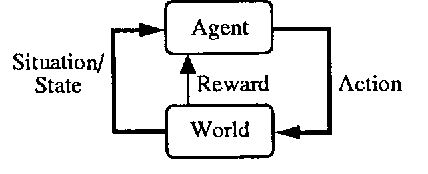
\includegraphics[angle=0,width=0.7\textwidth]{./figs/Dyna-Figure1.png}
		\caption{\label{fig:dyna}The Problem Formulation Used in Dyna. The agent's objective is to maximize the total reward it receives over time. \citep{Dyna}}
	\end{figure}

	\section{Reinforcement Learning}
	To further understand the underlying methods it is important to know the general mathematical rules and machine learning approaches. In the following, the terminology as well as mathematical background of the research subject is briefly summarized and explained. 
	%    \label{sec:rl}
	%    see Fig.~\ref{fig:image}    
	
	\subsection{Markov Decision Problem}
	A Markov Decision Problem (MDP) is a model for problems, where an agent tries to interact with the environment in such way that the utmost reward is achieved. Specifically, the robot is moving (\textit{transition}) through various \textit{states}, having chosen a specific \textit{action} in each state. Each \textit{reward} is determined by the initial state, the action, and the following state. 
	All transitions are not deterministic, but rather probabilistic, where each probability only depends on the current state and the current action. This memoryless property of stochastic processes is referred to as \textbf{Markov condition}. That way there has to be one initial state, but multiple end states are possible.\\
	\newpage The main goal is to find a reward maximizing \textbf{policy}, by which the agent selects actions where the maximum reward can be expected. This policy is an optimal plan, or sequence of actions, from start to a goal \citep{Lecture}.
	\par A Markov decision process consists of
	\begin{itemize}
		\item Set of states $S:$ $\{s_1,s_2,\dots, s_n\}$
		\item Set of actions $A:$  $\{a_1,a_2,\dots, a_n\}$ 
		\item Transition function, which is the probability of going from state $s$ to state $s'$ via action $a$: $T: S\times A \times S$
		\item  Reward function $R: S\times A \times S \rightarrow \mathbb{R}$
	\end{itemize}
	The main goal is to find an optimal policy $\Pi$ and exploration factor $\gamma$, where
	\begin{itemize}
		\item $\Pi$ is the policy, where an optimal action is assigned to each state
		\item $\gamma \in [0,1]$ is the discount factor. This factor determines the degree of exploration for the agent. For $\gamma=0$, the agent will stick to the policy, and exploit the current (possibly) optimal policy. For $\gamma=1$, the agent will take into account the next states' reward, leading to exploration behavior. A value $<1$ is a constraint, which limits the maximally obtainable reward, leading to a reduction of cycles.
	\end{itemize}
	The \textbf{V-values} and \textbf{Q-values} are certain grading schemes used to solve MDPs. The values are the total reward the agent can expect if it performs the optimal, or maximally benefitting, action $a$ in state $s$, and continues to act optimally thereafter:
	\begin{equation}\label{eq:vvalue}
	V^*(s) = \max_{a \in A} \sum_{s' \in S}^{} T(s,a,s')[R(s,a,s')+\gamma V^*(s')]
	\end{equation}
	As the values from equation \ref{eq:vvalue} are hard do compute, a technique called \textbf{value iteration} is used. It is used do discretize the equation: 
	\begin{equation}\label{eq:value-iteration}
	V^k(s) = \max_{a \in A} \sum_{s' \in S}^{} T(s,a,s')[R(s,a,s')+\gamma V^{k-1}(s')]
	\end{equation}
	where $k$ is the radius from the goal state to the agent. For example, regarding the Manhattan norm in a 2D plane, the amount of steps the agent has left until it reaches an end state.\\
	After that, \textbf{policy extraction} is performed. It is the assignment of an action to each state, maximizing the expected total reward:
	\begin{equation}
	\Pi^*(s) = \text{arg}\max_{a \in A} \sum_{s' \in S}^{} T(s,a,s')[R(s,a,s')+\gamma V^*(s')]
	\end{equation}
	\begin{figure}[t]
		\centering
		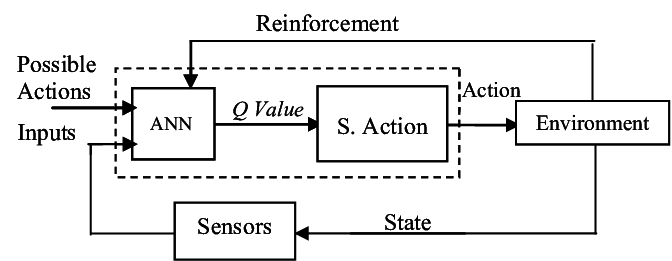
\includegraphics[angle=0,width=0.7\textwidth]{./figs/RL_ANN.png}
		\caption{\label{fig:qlearn}The structure of reinforcement learning based on an Artificial Neural Network \citep{HatemRL}}
	\end{figure}
	\subsection{Q-Learning}\label{sec:qlearn}
	Q-Learning is a model-free reinforcement learning algorithm which converges to optimal policy even if if the performed actions are suboptimal \citep{Lecture}. The letter \textbf{Q} stands for \textbf{quality} of a certain action in a given state, as the values represent the maximum discounted future reward when action $a$ in state $s$ is performed. Q-values are calculated similar to the value iteration in Equation \ref{eq:value-iteration}:
	\begin{equation}\label{eq:qlearn}
	Q^*(s,a) = \max_{a \in A} \sum_{s' \in S}^{} T(s,a,s')[R(s,a,s')+\gamma V^*(s')]
	\end{equation}
	The funcion $Q(s,a)$ can be estimated using Q-Learning, which is a form of \textbf{Temporal Difference Learning} (TD). TD means that an update is performed after every action based on a maximum reward estimate, and not only after receiving the reward.
	\par  Here, value $Q(s,a)$ is iteratively updated using the \textbf{Bellman Equation}: \\\\
	\begin{equation}\label{eq:qupdate}
	Q(s,a) \leftarrow Q(s,a) + \alpha [r + \gamma \max_{a' \in A}Q(s',a')-Q(s,a)]
	\end{equation}
	The Q-values are represented in a \textbf{Q-table} where each cell represents the highest achievable reward performing the state-action pair $(s\in S, a\in A)$. This makes Q-learning suitable for small environments only, as an increase in states or actions increases the amount of memory required to save and update that table $\mathcal{O}(n^2)$. The amount of time required to explore each state to create the required Q-table would be incredibly large.
	\par To counteract the use of large Q-tables for look-up, neural networks are used in \textbf{Deep Q-learning} (DQN) to approximate the Q-value function, where the state represents the network's input and the Q-values of all actions are its output.
	\par The challenge is to tune the parameters $\alpha , \gamma$ such that the best possible policy is found in minimal time.
	\subsubsection{Prioritized Sweeping}
	As mentioned in Section \ref{sec:qlearn}, the memory consumption of plain Q-Learning increases significantly with the amount of possible states and actions. Regarding large environments, the update of each value is extremely inefficient and time consuming.
	\par This is the idea behind \textit{prioritized sweeping}(PS) proposed by \citet{Moore93}. In PS, a queue is maintained of every state-action pair whose estimated value would have the most significant change. \citep{Sutton1998}. The Q-values are then updated multiple times, without actually performing any action. This is advantageous, since the execution of a movement usually takes more time than the calculations of the simulated actions, significantly shortening learning time.
	
	\section{GALMO}
	\begin{figure}[t]
		\centering
		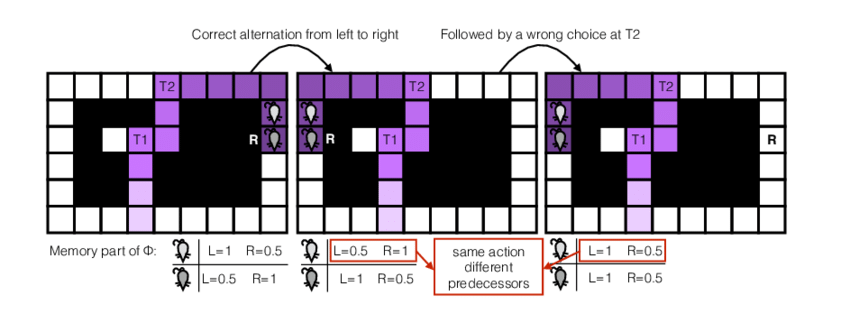
\includegraphics[angle=0,width=0.9\textwidth]{./figs/MultiplePredecessors.png}
		\caption{\label{fig:predecessors}Example of multiple predecessors in the alternation task. At the last position on the third run (right), the location component of the predecessor state (white mouse) is identical but the memory component is different. \citep{NeuralDynaQ}}
	\end{figure}
	\label{sec:galmo}
	\citet{NeuralDynaQ} encountered a problem when modelling the experimental environment, namely that under certain circumstances some states may have more than one predecessor, see Figure \ref{fig:predecessors}. This occurs especially during the third task, where reward sides alternate each lap.
	\par To confront this issue, \citet{NeuralDynaQ} created a growing type of algorithm called \textbf{GALMO}, an abbreviation for \textit{growing algorithm to learn multiple outputs}. This algorithm allows the creation of multiple neural networks $N_i$ so that multiple outputs can be generated for a single input. Each of the $N_i$ networks is coupled with a gating network $G_i$ deciding which network's output is considered for further calculations, see a schematic example on Figure \ref{fig:example}. The algorithm should also track the statistics of the minimal training errors of each sample to detect outliers. It is assumed that an outlier is caused by an input that should predict multiple outputs. GALMO then creates a new network based on a copy of the most suitable network for this input and trains it once. 
	\par The second part of the algorithm works as neural network-based Dyna-Q with prioritized sweeping. The rat moves in the maze environment and stores the samples in a priority queue, where the priority is the absolute value of the reward prediction error. At point of reward, replays are simulated given a certain budget, representing the phenomenon of hippocampal replays that occur in real-life situations \citep{OKEEFE1971171}. As expected, the higher prioritized samples are replayed first. Their predecessors are then estimated and placed back into the queue until budget exhaustion.\\
	The reason behind the implementation of a complex algorithm GALMO was to create a framework to analyze the role of hippocampal replays in the learning process, and whether there are patterns that can be observed in the artificial network which correspond to those in real neural networks.
	\begin{figure}[t]
		\centering
		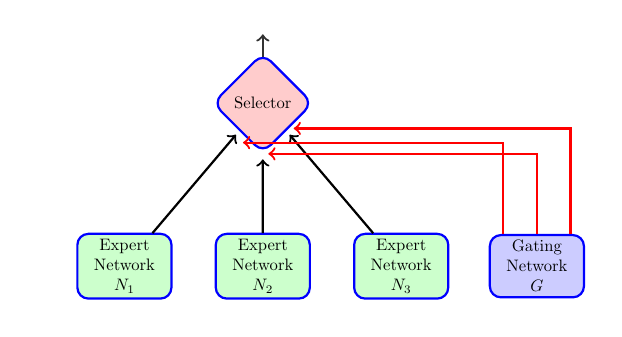
\begin{tikzpicture} [
		scale=0.6,  every node/.style={scale=0.6},
		block/.style    = { rectangle, draw=blue, thick, 
			fill=green!20, text width=5em, text centered,
			rounded corners, minimum height=2em },
		gate/.style    = { rectangle, draw=blue, thick, 
			fill=blue!20, text width=5em, text centered,
			rounded corners, minimum height=2em },
		outss/.style    = {diamond, draw=blue, thick, 
			fill=red!20, text width=4em, text centered,
			rounded corners, minimum height=1.5em },
		line/.style     = { draw, thick, ->, shorten >=2pt },
		]
		% Define nodes in a matrix
		\matrix [column sep=5mm, row sep=10mm] {
			
			& & \node [outss] (s) {Selector};  & &\\
			& \node [block] (n1) {Expert\\ Network\\ $N_1$}; & \node [block] (n2) {Expert\\ Network\\ $N_2$}; & \node [block] (n3) {Expert\\ Network\\ $N_3$}; & \node [gate] (g) {Gating\\ Network\\ $G$};\\
		};
		% connect all nodes defined above
		\begin{scope} [every path/.style=line]
		\path (n1)        --    (s) ;
		\path (n2)        --    (s);
		\path (n3)        --    (s);
		% Draw the links between gating
		\path[->,thick,red]
		([xshift=3mm] g.north west) |- ([yshift=-3mm] s.south west);
		\path[->,thick,red]
		([xshift=0mm] g.north) |- ([xshift=0mm] s.south);
		\path[->,thick,red]
		([xshift=-3mm] g.north east) |- ([xshift=0mm] s.south east);
		\path[->,thick,black!80]
		([yshift=-1mm] s.north) -- ([yshift=5mm] s.north);
		\end{scope}
		\end{tikzpicture}
		\caption{\label{fig:example}A system of expert and gating networks. Each expert as well as gating network is a feedforward network with same amount of inputs and outputs\citep{AdaptiveMixture}. Derived scheme.}
	\end{figure}
	
	\section{Project and Results}
	\label{sec:project}
	As part of practical work, a simplified T-maze configuration with a discrete environment similar to the work of \cite{NeuralDynaQ} has been reproduced, see Figure~\ref{fig:ui}. The programming language of choice was Python, as it offers many up-to-date machine learning libraries and allows a fast and understandable implementation. Helpful tutorials by \citet{harrison.2019} were used for orientation and knowledge acquisition in the present metier. 
	\par Again, the agent can choose between four actions: moving North, South, East and West. However, an extension was implemented where the agent can decide to run into the boundary. Although this does not change the position of the agent, it will be detected and punished with a higher penalty than the one for ``successful'' movement.\\
	\begin{figure}[b]
		\centering
		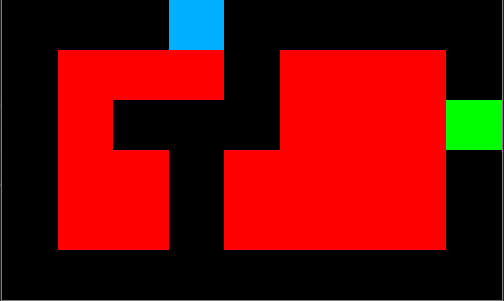
\includegraphics[angle=0,width=0.4\textwidth]{./figs/Environment.png}
		\caption{\label{fig:ui} Graphical display of the created environment. Blue: agent's position; green: the food pellet/reward; red: maze walls.}
	\end{figure}
	\par The environment was modified in such way that the tasks mentioned above can be executed. For task 1) and 2), the food pellet (\textit{reward}) was placed in a rigid position on the left or the right-hand side.  For the successful completion of task 3 (reward sides alternate) the state space was extended by two components: the left side reward memory (L) and the right side reward memory (R), as proposed by \citet{NeuralDynaQ}. They take a value 2 if the last reward was obtained on that side, 1 if the reward was obtained on that side the previous time, and 0 if there was no reward found on that side during the last 2 runs. \\
	Additionally, the starting point of the agent was moved from point S to decision point T1, see Figure \ref{fig:setup} for comparison. This step was necessary, otherwise the agent would have exploited the much shorter route around the maze walls, without ever passing through points T1 or T2.\\
	\par A posteriori, the efficiency of the developed environment model with the corresponding Q-learning has been compared with the Dyna-Q model with GALMO from \citet{NeuralDynaQ}. The present model is capable of learning every of the given tasks. The performance of task 1) and 2) were nearly identical since the distance to reward sides from starting position is identical left and right, see Figure \ref{fig:task12}. \\
	The resulting performance of the projects Q-learning implementation and the Neural Dyna-Q implementation were broadly reproduced. Both algorithms needed around 1000 episodes to converge, see proportion of errenous choices Figures \ref{fig:galmo},\ref{fig:task3}. The projects Q-learning converged around $30\%$ faster, but this is based on the fact that the path to rewarding pellets was reduced by about this percentage due to the changed initial placement of the agent. 
	\par Ultimately, this minimal improvement cannot keep up with the Neural DynaQ results of \citet{NeuralDynaQ}, since their implementation already converged after about 200 episodes, being five times more effective. 
%	Besides, there was a surprising conclusion that the performance of the projects Q-learning implementation and the advanced GALMO was quite similar as well, as both algorithms only needed about 200 episodes to converge, see Figures \ref{fig:task3},\ref{fig:galmo}.  
	
	\begin{figure}[t]
		\centering
		\begin{subfigure}{1\textwidth}
			\centering
			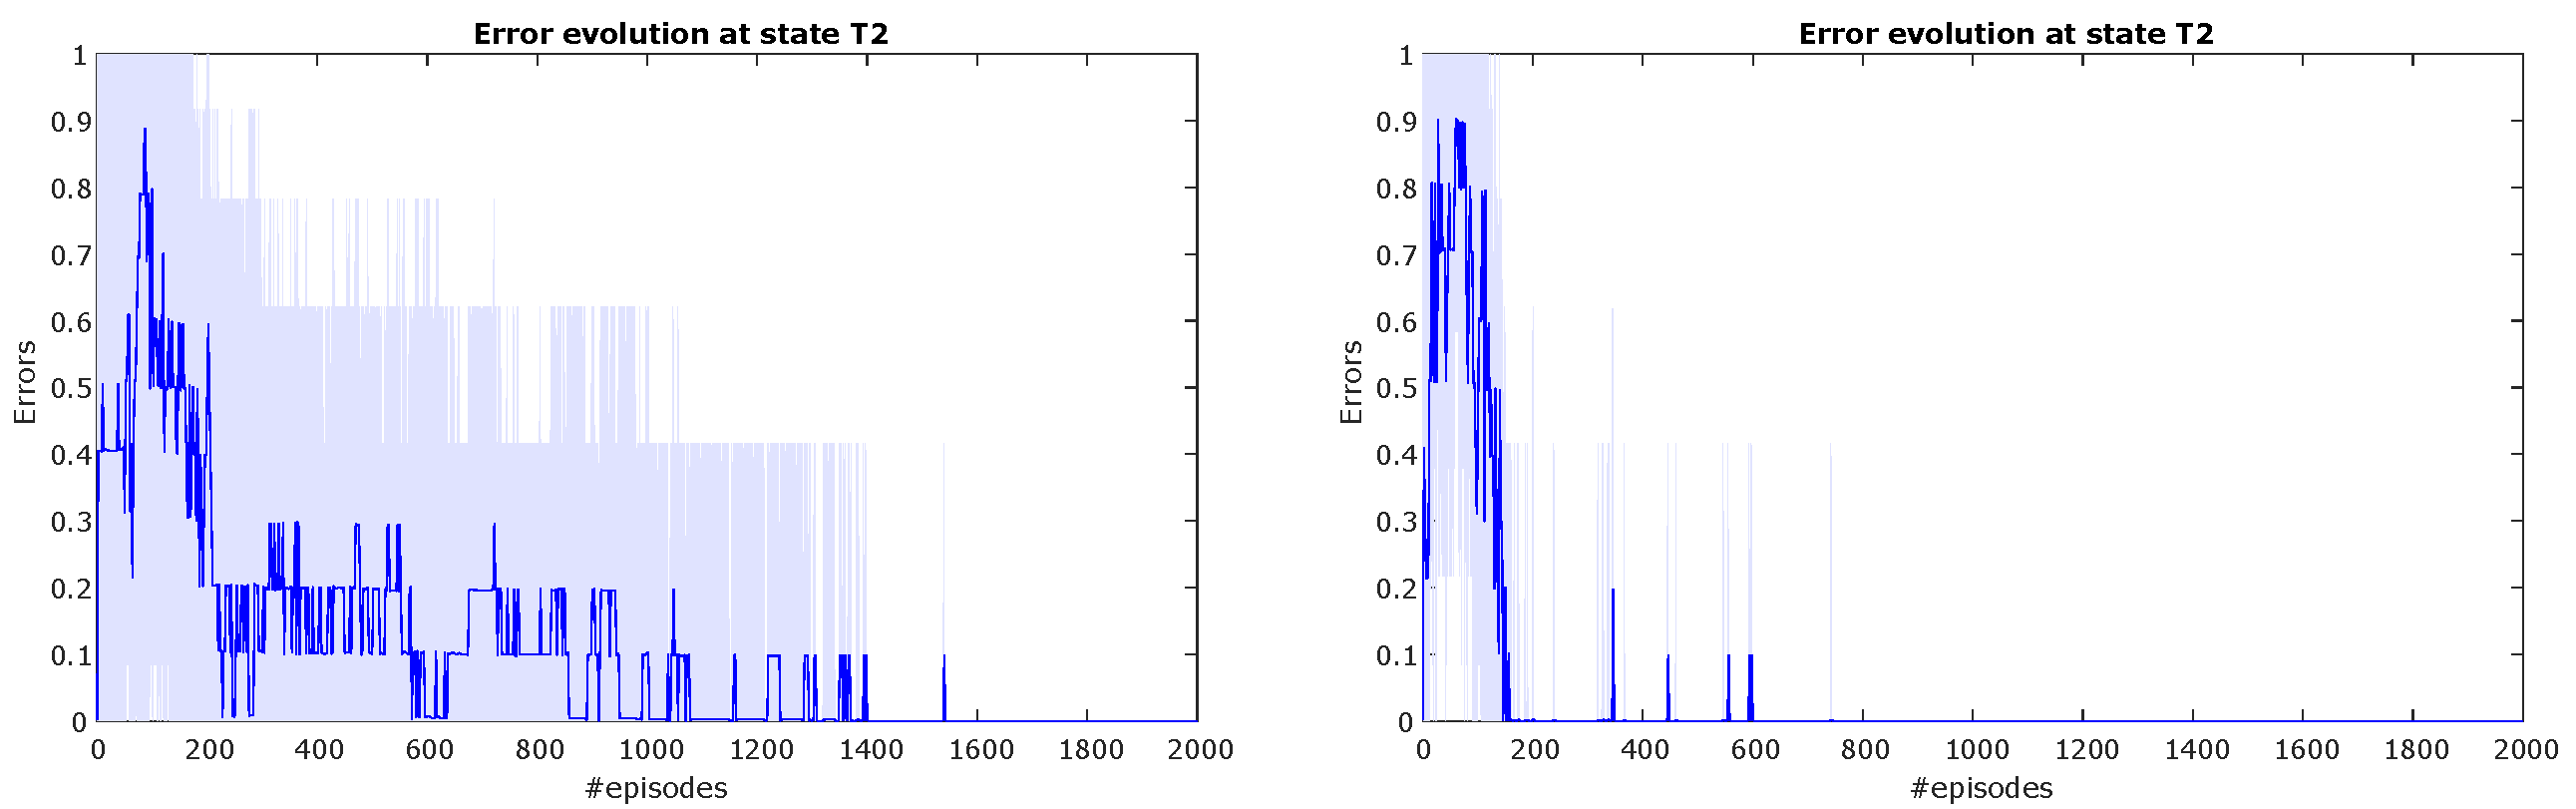
\includegraphics[height=4cm]{./figs/QvsDyna2.pdf}
			\caption{Learning without (left) and with (right) replays \citep{NeuralDynaQ}.}
			\label{fig:galmo}
		\end{subfigure}\\
		\begin{subfigure}{.4\textwidth}
			\hspace*{-1cm}
			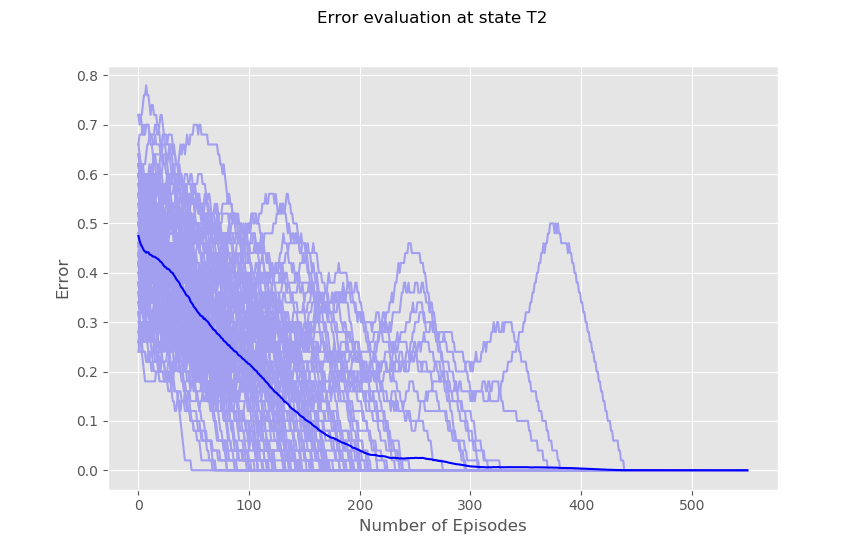
\includegraphics[height=4cm]{./figs/ErrorTask1.png}
			\caption{Performance during Task 1 in the project.}
			\label{fig:task12}
		\end{subfigure}
		\begin{subfigure}{.4\textwidth}
			\vspace*{-.4cm}
			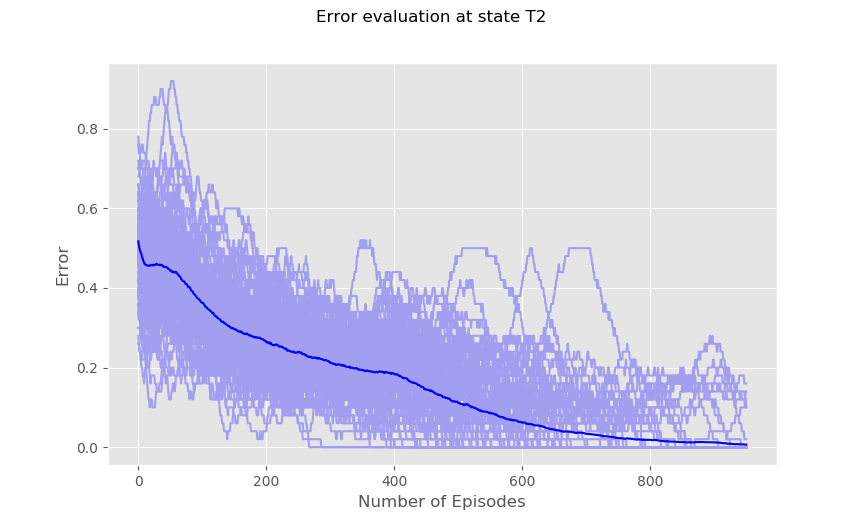
\includegraphics[height=4cm]{./figs/ErrorTask3.png}
			\caption{Performance during Task 3.}
			\label{fig:task3}
		\end{subfigure}\\
		
		\caption{\textbf{Learning dynamics of the own Q-learning implementation in comparison to GALMO performance}. Figures \ref{fig:task12},\ref{fig:task3} show the evolution of the proportion of decision errors at point T2 during Task 1 and Task 3, respectively.}
		\label{fig:tasks}
	\end{figure}
	\newpage
	\section{Conclusion}
	\label{sec:conclusion}
	In this paper the biological background of reinforcement learning was described. The current mathematical methods and approaches were reviewed, followed by a brief explaination of why associated implementation problems occur. \\
	A practical part was also created for this work, being Python implementation of Q-learning for a simple environment as well as its learning performance analysis. The results were very similar to the respective results of \citet{NeuralDynaQ}; there were small differences due to own minimal changes of the task.\\
	Concerning GALMO, \citet{NeuralDynaQ} would like to test the dynamic algorithm in a larger and more complex environment to better evaluate its functionality, since the used test environment was quite limited. It has been shown that the corresponding Neural DynyQ with prioritized sweeping performs five times better than the plain Q-learning implementation.\\
	\par Unfortunately, no information was given on the duration of the neural networks's learning phase, which would certainly be interesting considering a cost-benefit calculation. Especially since the project's Q-learning implementation for a simple environment requires only a few seconds until convergence.
	
	
	\footnotesize
	\bibliographystyle{plainnat}
	\bibliography{./main}
	\newpage
	%    \appendix
	%    \lstinputlisting[language=python, caption={Q-Learning in Python}]{../Code/QLearningOriginalEnv.py}
\end{document}
